\documentclass[aspectratio=43,display]{beamer}
%
% Choose how your presentation looks.
%
% For more themes, color themes and font themes, see:
% http://deic.uab.es/~iblanes/beamer_gallery/index_by_theme.html
%
\mode<presentation>
{
\usetheme{PaloAlto}      % or try Darmstadt, Madrid, Warsaw, ...
\usecolortheme{crane} % or try albatross, beaver, crane, ...
\usefonttheme{structurebold}  % or try serif, structurebold, ...
}

\usepackage{graphicx}
\usepackage{subfig}
\usepackage[brazil]{babel}
\usepackage[utf8x]{inputenc}
\usepackage{siunitx}
\usepackage{enumerate}
\usepackage{hyperref}
\usepackage{eso-pic}
\hypersetup{
bookmarksopen=false,
%pdfpagemode=UseNone,
pdfpagemode=FullScreen,   %% Enable to have Adobe Reader query for fullscreen mode
pdfauthor={André Luiz Abdalla Silveira} %% Enter the apppropriate author in here
}
\usepackage{dirtytalk}

\definecolor{prim}{HTML}{990000}
\definecolor{sec}{HTML}{FFCCCC}
\definecolor{ter}{HTML}{FFFFCC}
%\setbeamercolor{separation line}{bg=prim}
%\setbeamercolor{block title}{bg=prim, fg=white}
%\setbeamercolor{block body}{bg=sec, fg=black}

\newcommand\AtPagemyUpperLeft[1]{\AtPageLowerLeft{%
\put(\LenToUnit{0.75\paperwidth},\LenToUnit{0.89\paperheight}){#1}}}
\AddToShipoutPictureFG{
\AtPagemyUpperLeft{{
\includegraphics[width=.75cm,keepaspectratio]{../figuras/ime.png}}}
}%

\title[DELPo]{MAC 0499 -- Dicionário Etimológico da Língua Portuguesa}
%% Author with both abbreviation and affiliation
\author{André Luiz Abdalla Silveira}
\institute{Instituto de Matemática e Estatística \\ Universidade de São Paulo}
\date{\today}

\begin{document}
  \begin{frame}
    \maketitle
  \end{frame}

  \begin{frame}
    \tableofcontents
  \end{frame}

  \section{Introdução}\label{sec:introducao}

  \begin{frame}
    \tableofcontents[currentsection]
  \end{frame}

  \begin{frame}{O que é o DELPo}
    \begin{itemize}
      \item material de estudo de um TCC no ano passado \pause
      \item acrônimo de Dicionário Etimológico da Língua Portuguesa \pause
      \item projeto criado em 2012 pelo Prof. Dr. Mário Eduardo Viaro (DLCV -- FFLCH-USP) \pause
      \item destinado a facilitar o estudo de etimologia \pause
      \item plataforma processa textos recebidos e alimenta a base de dados
    \end{itemize}
  \end{frame}

  \begin{frame}{Funcionalidades}
    \begin{itemize}
      \item Moedor -- principal e foco da refatoração \pause
      \item Metaplasmador \pause
      \item Analisador de frequência ao longo dos anos
    \end{itemize}
  \end{frame}

  \section{Propostas}\label{sec:propostas}

  \begin{frame}{Propostas}
    \tableofcontents[currentsection]
  \end{frame}

  \subsection{Interface de usário}\label{subsec:interface}

  \begin{frame}{A camada de apresentação}
    \begin{itemize}
      \item A aplicação funcionava, mas a interface feita estava sem estilização alguma \pause
      \item ActiveViewer (Rails) $\rightarrow $ Nuxt.js % 2 camadas de aplicação -- não gera mais trabalho?
      \begin{itemize}
        \item facilidade de uso \pause
        \item flexibilidade  \pause %trade off
        \item menos \say{poluição} no controlador \pause
      \end{itemize}
      \item Aplicação Rails no modo API
    \end{itemize}
  \end{frame}

  \subsection{Testes}\label{subsec:testes}

  \begin{frame}{Testando as aplicações}
    \begin{itemize}
      \item permitem verificar o funcionamento (ou não) do código \pause
      \item pressupõe que o testador conheça o código \pause % forçaram-me a desbravar o código
      \item O que se pode verificar?
      \begin{itemize}
        \item Comportamento da aplicação --- Rails (testes em RSpec) \pause % familiarizado
        \item Integração de componentes --- Nuxt (testes em Jest) \pause % preciso conhecer -- escolhi por ser mais acessível e parecido com o RSpec
      \end{itemize}
      \item Cobertura de testes na aplicação Rails: $72\%$ \pause % siimple-cov gem
      \item Cobertura de testes na aplicação Nuxt: Não haviam testes  % a própria ferramenta aponta a cobertura sem precisar de helpers
    \end{itemize}
  \end{frame}

  \subsection{Refatoração}\label{subsec:refatoracao}

  \begin{frame}{Melhorando o código}
    \begin{itemize}
      \item única das propostas a não estar na apresentação inicial \pause
      \item \say{Cheiros} do código nunca foram tão incômodos \pause % maioria dos alunos não tem uma ideia de quão catastrófico pode ser manter um código ruim, mas mexer com o código macarrônico alheio com certeza alerta a pessoa quanto a isso
      \item Motivos prováveis \pause
      \begin{itemize}
        \item Pressa para cumprir prazos \pause % limitam a qualidade do código
        \item Falta de expreriência de mercado com Rails \pause % isso me fez uma santa diferença --- muita coisa poderia ser usada e não foram
      \end{itemize}
      \item refatorar o código não quer dizer que o código é ruim \pause % algo bom pode sempre ser aperfeiçoado
      \item é benéfico à aplicação \pause
      \begin{itemize}
        \item tornou-a mais organizada, mais inteligível, e por isso, mais escalável \pause % reaproveitar a imagem do poster de comparação
        \item exemplos: criação de \emph{helpers} e uso de serializadores (transformam conjuntos de dados em um JSON)
      \end{itemize}
    \end{itemize}
  \end{frame}
  %interessante mencionar que a proposta subliminar era manter e melhorar o que já estava feito e entregar algo o mais funcional possível

  \begin{frame}{Exemplo de refatoração}
    \begin{figure}
      \centering
      \subfloat[\texttt{Antes}]{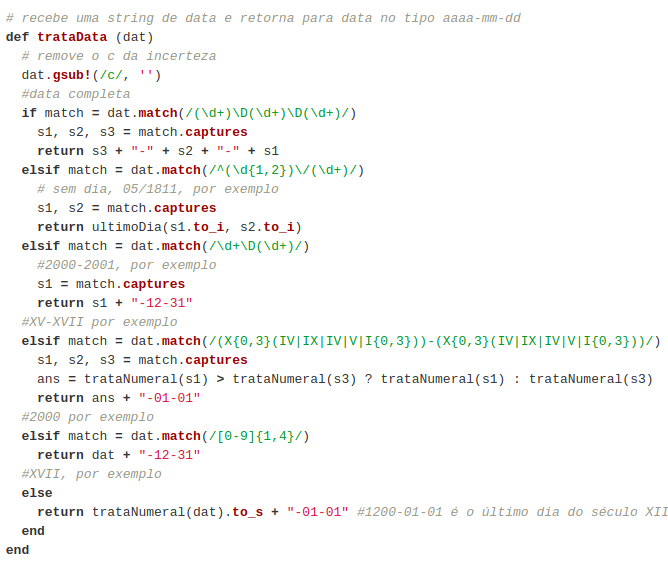
\includegraphics[width=.55\textwidth]{../figuras/antes.png}}
      \subfloat[\texttt{Depois}]{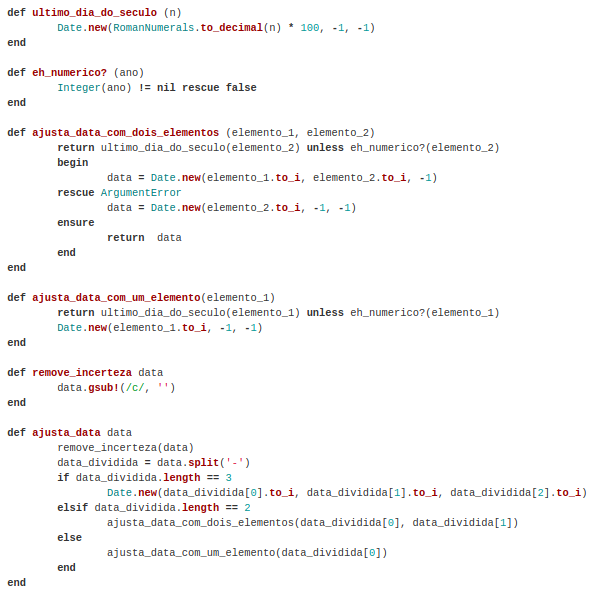
\includegraphics[width=.45\textwidth]{../figuras/depois.png}}
      \caption{Exemplo tirado do \texttt{DataHelper}}
    \end{figure}
  \end{frame}

  \section{Resultados}\label{sec:resultados}

  \begin{frame}{O que foi feito?}
    \tableofcontents[currentsection]
  \end{frame}

  \subsection{API}

  \begin{frame}{API}
    \begin{itemize}
      \item Foco em \say{despoluir} os controladores \pause
      \item Uso da gema \texttt{active\_model\_serializers} \pause
    \end{itemize}
    \begin{figure}
      \centering
      \subfloat[\texttt{Antes}]{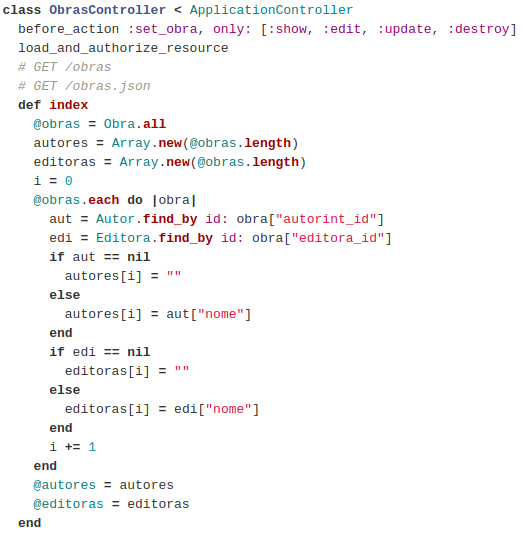
\includegraphics[width=.4\textwidth]{../figuras/obras_antes.png}}
      \subfloat[\texttt{Depois}]{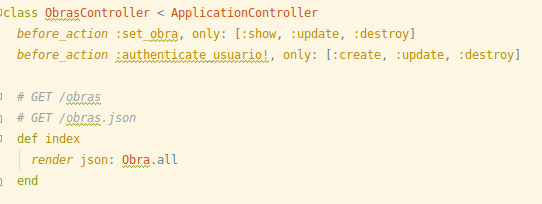
\includegraphics[width=.6\textwidth]{../figuras/obras_depois.png}}
      \caption{Exemplo tirado do \texttt{ObrasController}}
    \end{figure}
    %print do controlador de obras antes e depois e talvez o resultado de uma busca
  \end{frame}

  \begin{frame}{Serializer}
    \begin{figure}
      \centering
      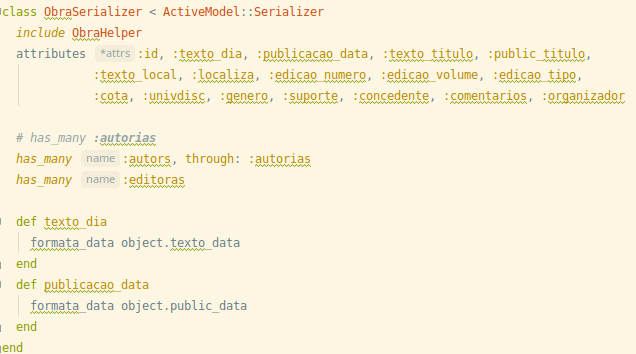
\includegraphics[width=.9\textwidth]{../figuras/obra_serializer.png}
      \caption{\texttt{ObrasSerializer}}
    \end{figure}
  \end{frame}

  \begin{frame}{Requisição}
    \begin{figure}
      \centering
      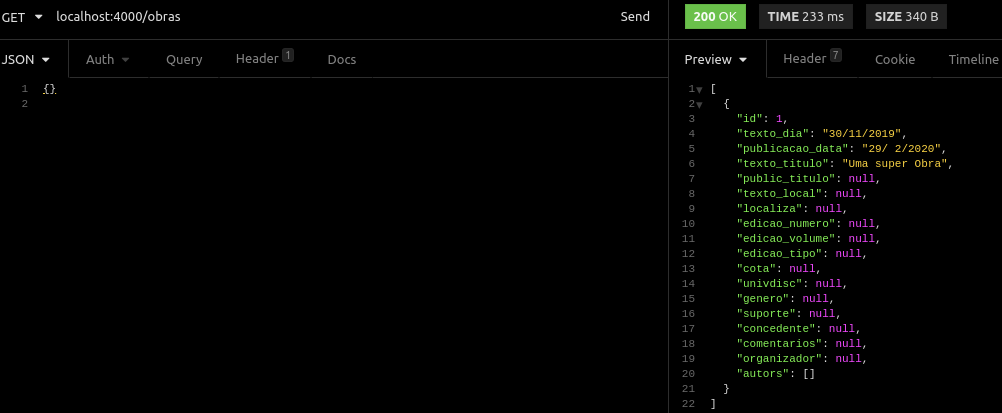
\includegraphics[width=\textwidth]{../figuras/get_obras.png}
      \caption{Resposta à requisição \texttt{\textbf{GET} localhost:4000/obras}}
    \end{figure}
  \end{frame}

%  \subsection{O moedor}\label{subsec:o-moedor}
%
%  \begin{frame}{Refatoração do moedor}
%    \begin{itemize}
%      \item Foco: quebrar métodos grandes de modo a torná-los mais compreensíveis e mais fáceis de testar
%      % muito código que fazia ourtas coisas como produzir e parsear datas estavam no model Moedor
%    \end{itemize}
%    %reaproveitar print do poster
%  \end{frame}

  \subsection{Interface}

  \begin{frame}{Camada de Apresentação}
    \begin{itemize}
      \item Conteúdos estáticos já estão prontos \pause
      \item Uso da ferramenta Vuetify. Um plug-in feito para Vue.js e seus derivados e que usa Material Design.
      \begin{itemize}
        \item Segundo o site \href{https://material.io/design/introduction/}{\textbf{https://material.io/design/introduction/}},
        é um paradigma que une princípios clássicos do bom design com a inovação da tecnologia e ciência. \pause
      \end{itemize}
      \item Foco: interligar com a API além do sistema de login \pause
      % a dificuldade que havia com o CORS foi superada com a ultilização da lib @nuxtjs/proxy
    \end{itemize}
    \begin{figure}[htb]
      \centering
      \subfloat[\texttt{/home}]{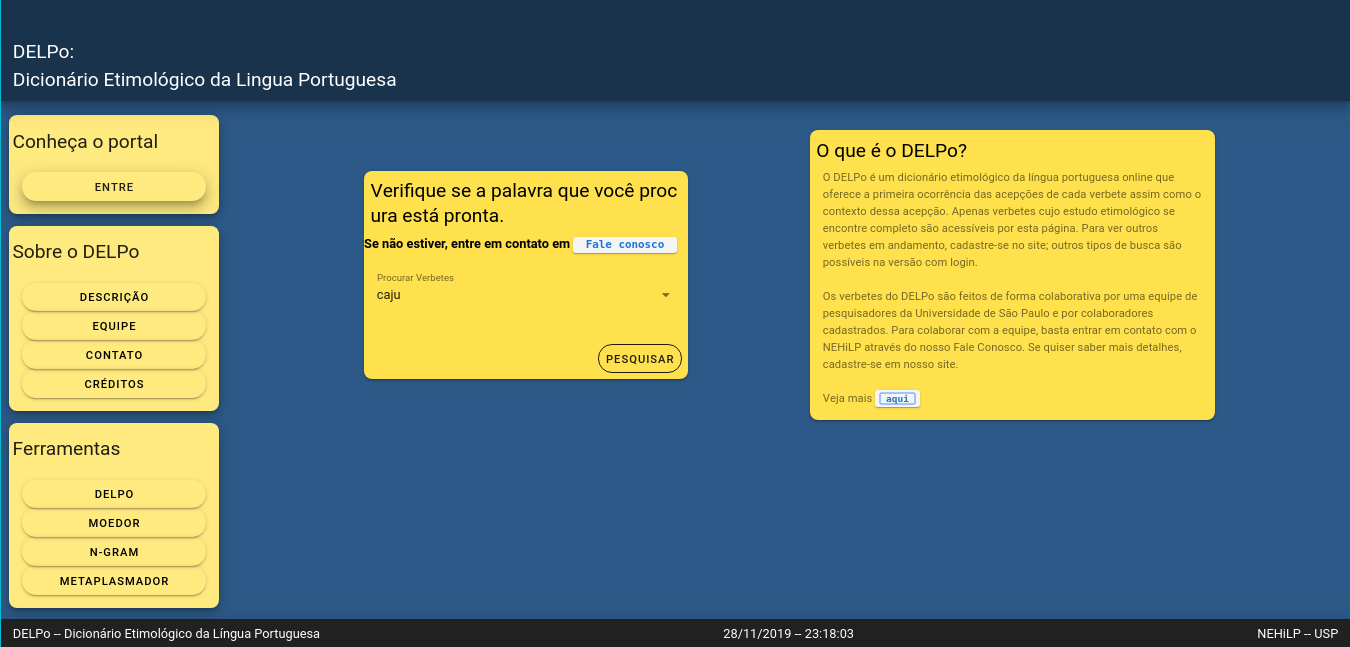
\includegraphics[width=.5\textwidth]{../figuras/home.png}}
      \subfloat[\texttt{/equipe}]{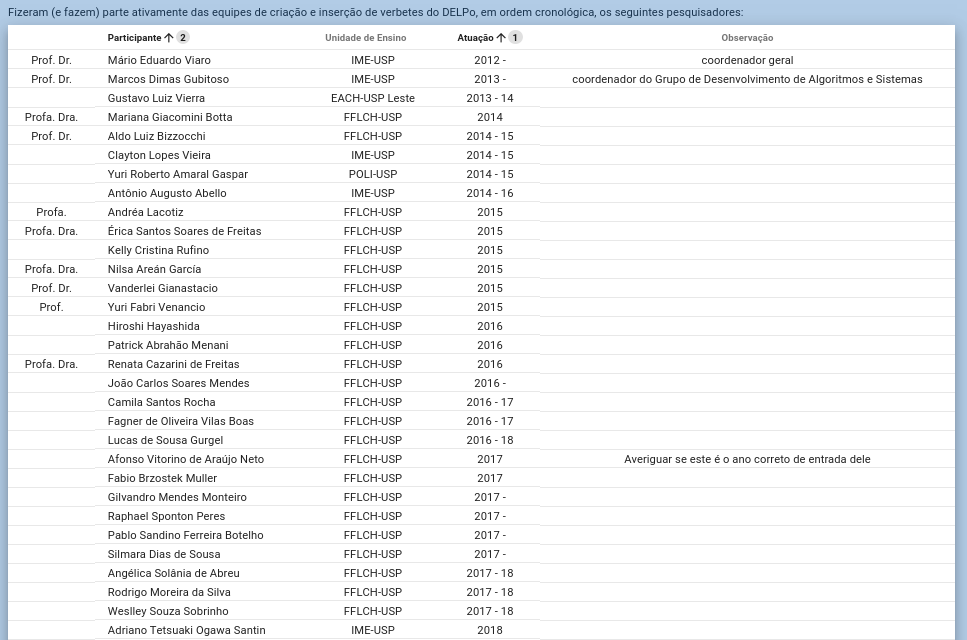
\includegraphics[width=.35\textwidth]{../figuras/lista_pesquisadores.png}}
      \caption{Captura de telas feitas a partir da interface}
    \end{figure}
    % oferecer-se a mostrar funcionando as demais rotas --  falar de bug no login
  \end{frame}

  \subsection{Balanço Geral}

  \begin{frame}{Atividades}
    \begin{itemize}
      \item Concluídas
      \begin{itemize}
        \item Refatorar o banco de dados \pause
        \item Refatoração dos modelos e controladores \pause
        \item Modularização das classes e interfaces \pause
      \end{itemize}
      \item Em Andamento
      \begin{itemize}
        \item Fazer uma interface de usuário agradável (60\%) \pause
        \item Fazer os testes no back (73\%) \pause
        \item Refatoração do moedor (70\%) \pause
      \end{itemize}
      \item Não Iniciadas
      \begin{itemize}
        \item Adaptação dos dados do banco de dados antigo \pause
        \item Fazer os testes do front \pause
      \end{itemize}
      \item Observação: As porcentagens na coluna do meio são uma estimativa do grau de conclusão da tarefa
    \end{itemize}
  \end{frame}

  \section{Aprendizados}\label{sec:aprendizados}

  \begin{frame}{O que aprendi?}
    \begin{itemize}
      \item A importância do bom código \pause
      \item Equilíbrio entre a vontade de fazer o melhor e terminar determinadas tarefas
    \end{itemize}
  \end{frame}

  \section{Bibliografia}\label{sec:bibliografia}

  \begin{frame}{Publicações}
    \begin{itemize}
      \item O dicionário etimológico da língua portuguesa (delpo): conceitos de metalema, hemilema, hiperlema e
      ultralema --- Mário Eduardo Viaro --- 2017
      \item Boas práticas --- Daniel Schmitz --- 2019
      \item Refatoração do Projeto Delpo --- Adriano Tetsuaki Ogawa Santin, Luiz Fernando Antonelli Galati e
      Mauricio Luiz Abreu Cardoso --- 2018
      \item O uso do dicionário de língua como instrumento didático no ensino de língua portuguesa para alunos
      surdos: em busca de um bilinguismo funcional --- Barbara Neves Salviano --- 2014
      \item Clean code --- Wojtek Lukaszuk --- 2018
      \item Ruby Cookbook --- Lucas Carlson e Leonard Richardson --- 2009
      \item Manual do NEHiLP
    \end{itemize}
  \end{frame}

  \begin{frame}{Documentações}
    \begin{itemize}
      \item Ruby on Rails Guides
      \item Vue.js Docs
      \item Nuxt.JS Guide
      \item Jest Homepage
    \end{itemize}
  \end{frame}

\end{document}
